\section{Análisis}

A la hora de experimentar, utilizamos nuestra implementación de traceroute sobre diversas universidades de todo el mundo, analizando distintas distancias y cantidades de saltos intercontinentales.

\subsection{China}

El primer análisis se hizo sobre la Universidad de Tsinghua en Pekín, República Popular de China. Su dirección web es \url{www.tsinghua.edu.cn}, la cual resolvía la dirección IP 166.111.4.100 a la hora de la experimentación. Debido a su lejanía, su análisis resulta interesante.

De los 28 saltos que se produjeron en el trazado, solamente 3 de ellos no generaron una respuesta, lo cual representa aproximadamente 10\% de los hosts. Los mismos se trataron de los primeros saltos, por lo que creemos que son hosts del ISP que no responden a este protocolo. Si ignoramos estos saltos nos queda una trayectoria con una longitud de 25 saltos.

En el mapa podemos ver un total de 3 saltos intercontinentales. Las direcciones IP fueron geolocalizadas usando los distintos servicios anteriormente nombrados. Resaltamos las direcciones IP 185.70.203.32 y 89.221.41.187, las cuales representan los host de los saltos 9 y 10 respectivamente. Para estas direcciones, hay servicios de geolocalización que dicen que ambas se encuentran en Italia, pero existen otros servicios que la ubican a la primera en Argentina y a la segunda en EE.UU. Estas direcciones IP pertenecen a la empresa Telecom Sparkle, originaria de Italia. Esta se encarga de mantener cables marinos, por lo que realmente no sabemos si realmente se encuentran en Italia o si algunos servicios la marcan como italiana solo por ser una empresa de dicho país.

Aplicando el método de Cimbala a la diferencia entre RTTs promedio de cada salto, detectamos como outliers los saltos con las correspondientes TTLs, 10 (89.221.41.187), 13 (154.54.84.1), 14 (154.54.30.162), 16 (154.54.44.86) y 19 (101.4.117.169). Lo primero que vimos es que el salto 9 no aparece como outlier, por lo que podríamos asumir que las direcciones IP tomadas como italianas tienen dicha localización por el origen de la empresa. Los saltos 13, 14 y 16 son saltos dentro de los Estados Unidos, por lo que podemos decir que el método introdujo falsos positivos. Finalmente el otro salto intercontinental desde norteamérica hacia asia fue el salto 19. Cuando aplicamos el método de  forma no iterativa, solamente nos toma como outliers los puintos que realmente representan saltos intercontinentales, donde los RTTs incrementan de forma muy marcada.

\subsection{Inglaterra}

Este experimento corresponde a la Universidad de Oxford, Inglaterra. Más especificamente, nuestro traceroute es a la dirección \url{www.ox.ac.uk}.

De los 27 hops que observamos hubo 7 que no respondieron Time Exceeded, es casi el 26 \% de los host. 3 hosts pertenecen al cluster correspondiente a Argentina, otros 3 a Estados Unidos y el último a Inglaterra.

Aqui podemos observar el recorrido trazado en el planisferio.

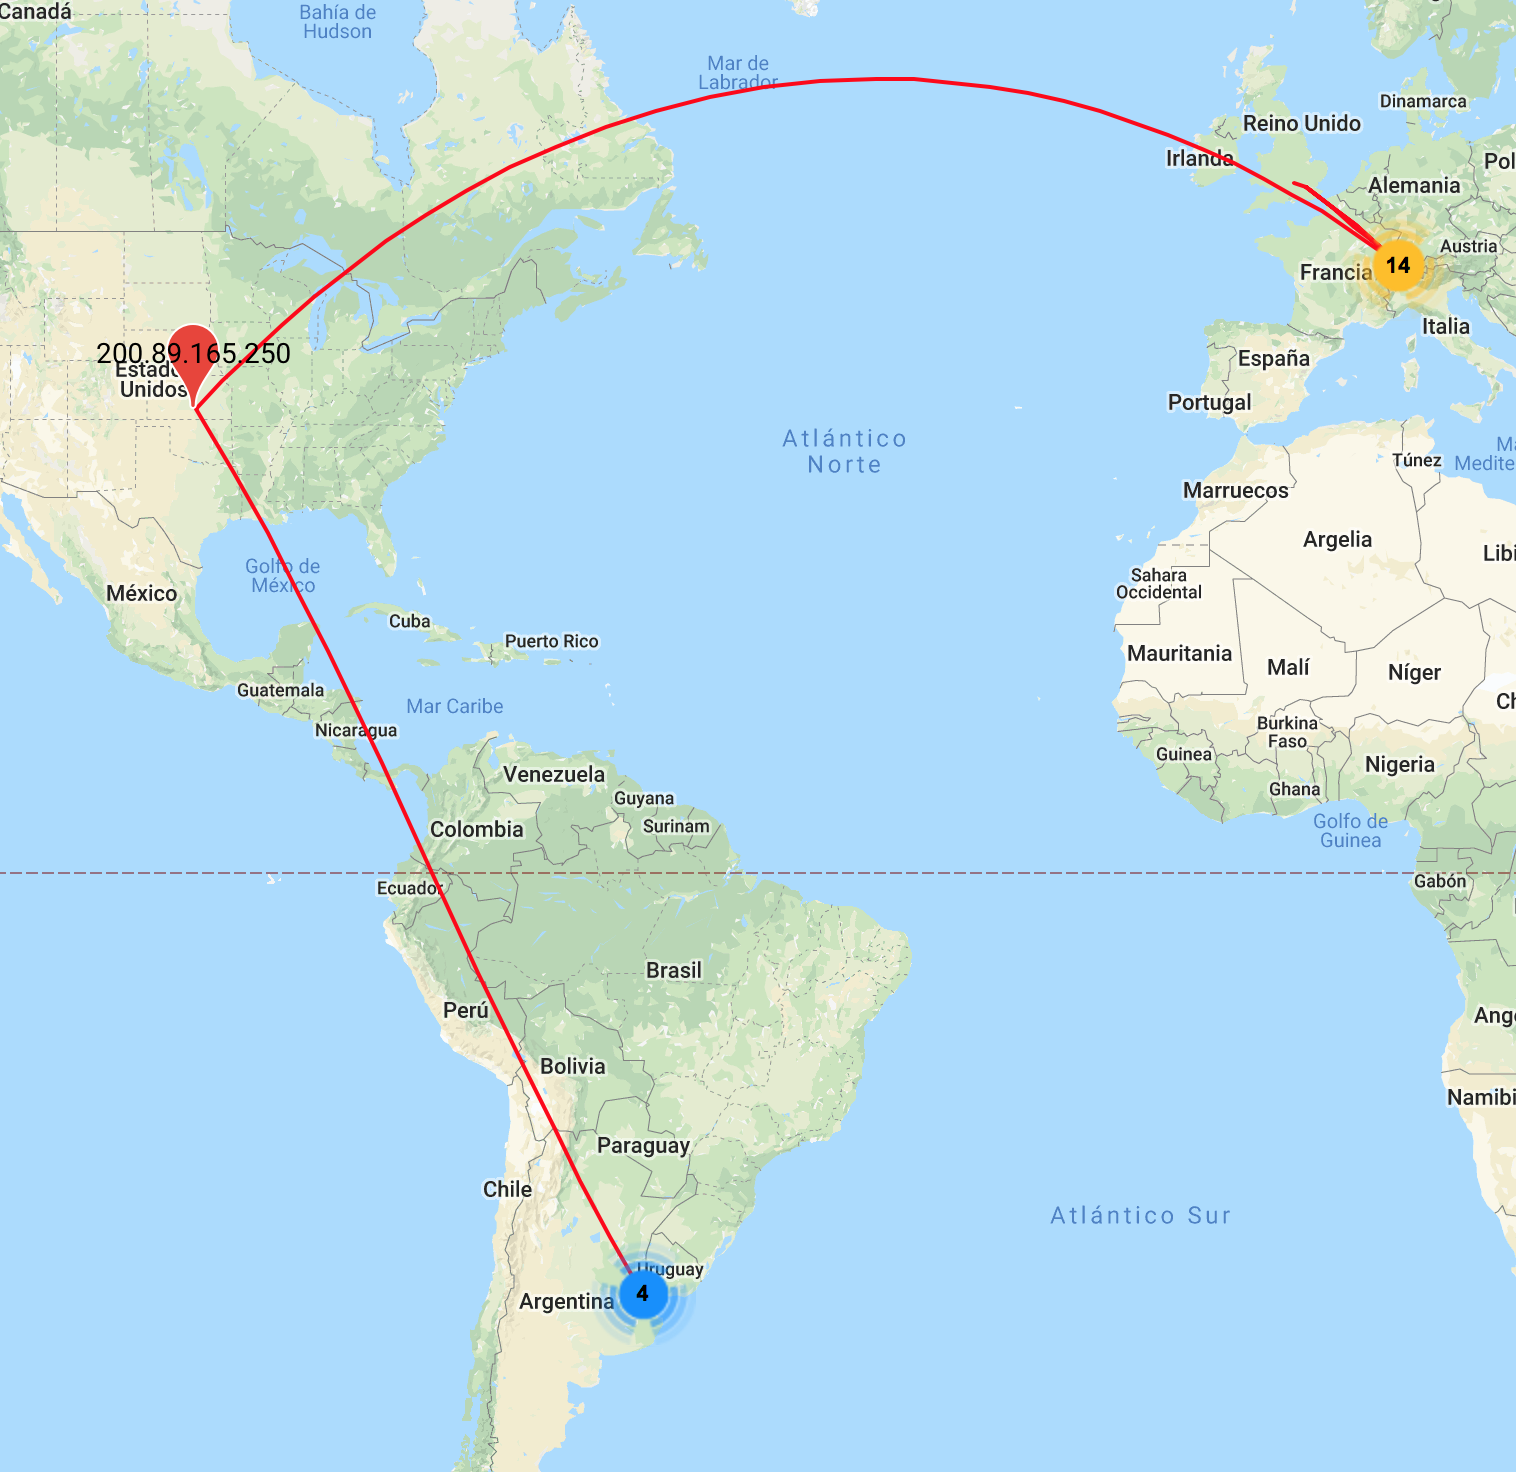
\includegraphics[width=\textwidth]{oxford_mapa.jpg}

Al geolocalizar los hosts con nuestros servicios, en el planisferio se observa una ruta con 2 enlaces intercontinentales. Además nos llamó la atención el hecho de que se realice un salto hacia Estados Unidos existiendo un cable submarino desde Brasil a Portugal. Pensamos que podria deberse a que es el único de Sudamérica hacia Europa y podría estar congestionado, mientras que desde Estados Unidos a Europa existen una cantidad considerable de enlaces submarinos.

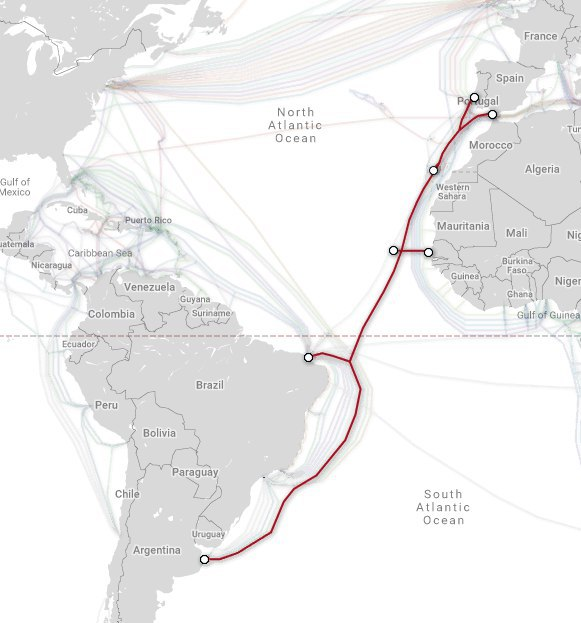
\includegraphics[width=\textwidth]{submarine_cable.jpg}

La distribución de RTT entre saltos presenta 3 outliers según el método Cimbala, lo cual no concuerda con la cantidad de saltos transoceánicos que se efectúan, que eran 2. El falso positivo es un salto que se produce dentro del cluster de argentina, la dirección  200.89.165.86
